\documentclass[]{BasiliskReportMemo}


\newcommand{\submiterInstitute}{Autonomous Vehicle Simulation (AVS) Laboratory,\\ University of Colorado}
\newcommand{\ModuleName}{simpleNav}
\newcommand{\subject}{Unit Test Results for Simple Navigation Model}
\newcommand{\status}{Initial Test Results}
\newcommand{\preparer}{S. Piggott}
\newcommand{\summary}{
   This is a report documenting the results of the Simple Navigation Model unit test created for 
   the AVS Basilisk Simulation as part of the EMM project. }


\begin{document}


\makeCover


%
%	enter the revision documentation here
%	to add more lines, copy the table entry and the \hline, and paste after the current entry.
%
\pagestyle{empty}
{\renewcommand{\arraystretch}{2}
\noindent
\begin{longtable}{|p{0.5in}|p{4.5in}|p{1.14in}|}
\hline
{\bfseries Rev}: & {\bfseries Change Description} & {\bfseries By} \\
\hline
Draft & Initial Revision & S. Piggott \\
\hline

\end{longtable}
}

\newpage
\setcounter{page}{1}
\pagestyle{fancy}

\tableofcontents
~\\ \hrule ~\\

%\begin{figure}[htb]
%	\centerline{
%	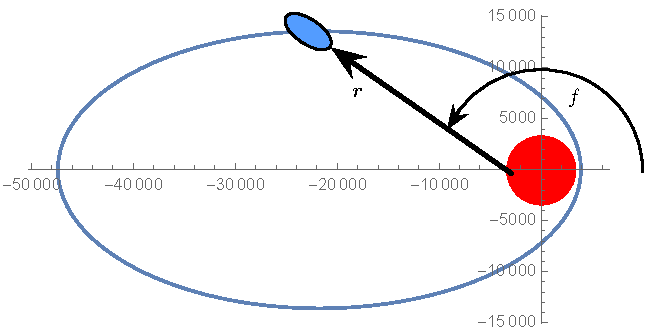
\includegraphics[]{Figures/Fig1}
%	}
%	\caption{Sample Figure Inclusion.}
%	\label{fig:Fig1}
%\end{figure}

\section{Introduction}
The Simple Navigation model in the AVS Basilisk simulation is used to generate 
a stand-in for the real navigation system.  Its use-case is to provide realistic 
navigation signals that are right at the spec of what ADCS claims for navigation 
system performance.  For a typical spacecraft navigation system, the spec will 
almost always be at least a factor of two lower in performance than the expected 
nominal capabilities of the on-board navigation system.  Therefore, we require 
the existence of a model that can provide spec-level navigation errors so that 
the functionality of the guidance and control subsystems can be verified as 
acceptable in the presence of navigation errors that are right at the spec. \\

The noise present in the simple navigation is designed to mimic the error signals 
that will be observed in the real navigation system.  The true "noise" present 
in a vehicle's navigation system is always a combination of bias, white noise, 
and brown noise (or random walk).  In order to provide this, a second-order 
Gauss-Markov process model was added to the simulation utilities that allows 
the user to configure a random walk process.  The output of this model when 
applied to the vehicle position can be observed in Figure~\ref{fig:pos_fig}.
\begin{figure}[htb]
        \centerline{
        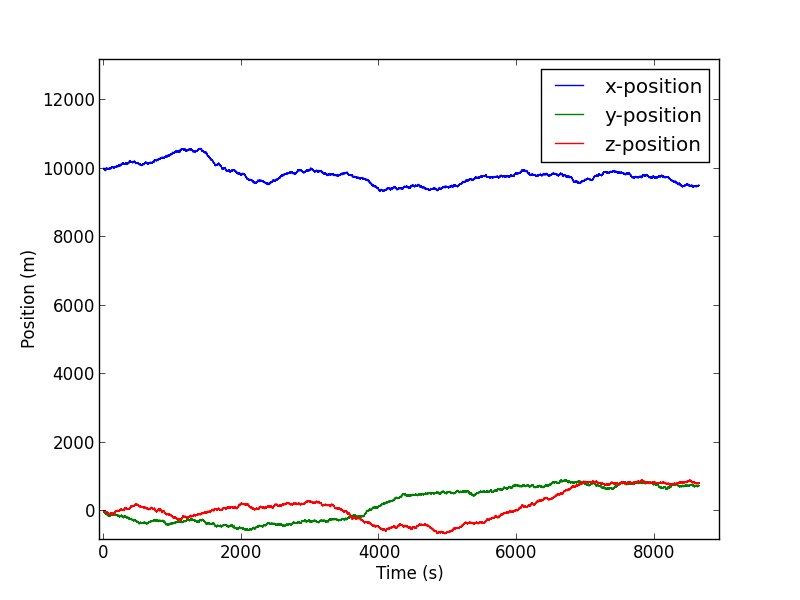
\includegraphics[scale=0.5]{Figures/SimpleNavPosition}
        }
        \caption{Simple Navigation Position Signal}
        \label{fig:pos_fig}
\end{figure} 

In this figure, the nominal position that the error was being distributed about
 was [10000.0, 0.0, 0.0] in meters and the error was bounded such that the 
absolute value of the error was less than 1000 m.  The random walk had a white 
noise standard deviation of 10 meters.

In the model, the vehicle position, velocity, attitude, attitude rate, 
accumulated delta-velocity, and sun-pointing vector have errors applied 
separately.  Arguably the sun-pointing vector should just use the vehicle 
attitude and the Sun position to get is pointing accuracy, but the Sun can be 
sensed independently of this and that is why there is a separate error source
used for it.

The top-level model relies on a lower-level utility module called GaussMarkov 
that supplies the random walk process that is added to the truth states.  
Since the simple\_nav model exercises this utility completely, the unit test 
documented here was also used to test the GaussMarkov model both in terms of 
functionality and in terms of code coverage.  The coverage results are included 
in a table in the results.

\section{Test Design}
The unit test for the simple\_nav module is located in:\\

\noindent
{\tt SimCode/navigation/simple\_nav/UnitTest/SimpleNavUnitTest.py} \\
\\

\noindent This unit test is designed to functionally test the simulation model 
outputs as well as get complete code path coverage.  The test design is broken 
up into three main parts:\\
\begin{enumerate}
\item{Error Bound Enforcement: The simulation is run for 2.4 hours and the 
   error bounds for all of the signals }
\item{Error Bound Usage: The error signals are checked for all of the model 
   parameters over the course of the simulation to ensure that the error gets 
   to at least 75\% of its maximum error bound at some point to make sure that 
   it isn't stuck around zero.}
\item{Corner Case Check: The simulation is intentionally given bad inputs to 
   ensure that it alerts the user and does not crash.}
\end{enumerate}


\section{Test Results}
\begin{enumerate}
\item{Error Bound Enforcement: We do want to violate the error bound a 
   statistically small number of times as most bounds are specified 3-sigma 
   and we'll need to be at the spec to make sure it works.  All signals remained 
   inside their bounds greater than 1-sigma (~0.3\%) of the time.  Check 
   successful. }
\item{Error Bound Usage: As stated above, we want to ensure that the random 
   walk process is effectively utilizing the error bound that it has been 
   given and not remaining mired near zero.  All error signals cross up above 
   75\% of their error bound at least once.  Check successful.}
\item{Corner Case Usage: All errors/warnings were stimulated and the simulation 
   still ran without incident.  Check successful.}
\end{enumerate}

\section{Test Coverage}
The method coverage for all of the methods included in the simple\_nav 
module are tabulated in Tables~\ref{tab:cov_met} and \ref{tab:cov_met2}.

\begin{table}[htbp]
    \caption{Simple Navigation Test Analysis Results}
   \label{tab:cov_met}
        \centering \fontsize{10}{10}\selectfont
   \begin{tabular}{c | r | r | r} % Column formatting, 
      \hline
      Method Name    & Unit Test Coverage (\%) & Runtime Self (\%) & Runtime Children (\%) \\
      \hline
      UpdateState & 100.0 & 0.08 & 15.0 \\
      SelfInit & 100.0 & 0.0 & 0.0 \\
      CrossInit & 100.0 & 0.0 & 0.0 \\
      computeOutput & 100.0 & 0.0 & 0.0 \\
      \hline
   \end{tabular}
\end{table}

\begin{table}[htbp]
    \caption{GaussMarkov Test Analysis Results}
   \label{tab:cov_met2}
        \centering \fontsize{10}{10}\selectfont
   \begin{tabular}{c | r | r | r} % Column formatting, 
      \hline
      Method Name    & Unit Test Coverage (\%) & Runtime Self (\%) & Runtime Children (\%) \\
      \hline
      computeNextState & 100.0 & 0.71 & 12.4 \\
      setRNGSeed & 100.0 & 0.0 & 0.0 \\
      setPropMatrix & 100.0 & 0.0 & 0.0 \\
      getCurrentState & 100.0 & 0.0 & 0.0 \\
      setUpperBounds & 100.0 & 0.0 & 0.0 \\
      setNoiseMatrix & 100.0 & 0.0 & 0.0 \\
      setPropMatrix & 100.0 & 0.0 & 0.0 \\
      \hline
   \end{tabular}
\end{table}
For all of the code this test was designed for, the coverage percentage is 
100\%.  The CPU usage of the model is higher than would be ideal although this 
might just be a symptom of the level of simplicity present in the overall 
simulation.  The majority of the computations are coming from two pieces of the 
GaussMarkov code.  

The first is the random number generator.  The model is using 
one of the simplest random number generators in the standard template library.  
That is still a relatively expensive operation as random numbers are costly and 
we generate a new random number for each state.  The second factor is in the 
state and noise propagation.  Those are being performed with a matrix 
multiplication that is an $n^2$ operation.  We could save some computations 
here in the future if we took away the cross-correlation capability from some 
of the states which would definitely be easy and accurate.  It would just take 
some more code.

\section{Conclusions}
The simple\_nav module is arguably complete.  That is a pretty lukewarm 
endorsement.  It is certainly complete from a PDR capability standpoint.  
However there are two areas of concern that may be worth addressing in the 
run-up to CDR.  The first is the boundary enforcement in the GaussMarkov 
source.  Right now it just does a rough "closeness" check that it then uses 
to exponentially pull the signals back inside the bound as they get close.  
Ideally we would use the statistical likelihood of a call cross the bound and 
then use that to pull the resultant random number away from it.  That would be 
slightly more robust but would require another non-trivial piece of code 
(error function).

The second issue is just processing.  15\% is a lot of CPU for the simple 
navigation model to be using.  However for a lot of sims and pretty much all 
post-CDR analysis we probably won't be using it for much and certainly not at 
a high rate so we can probably live with the CPU hit indefinitely.

\end{document}
